\documentclass[compress,handout]{beamer}

\usetheme[block=fill]{metropolis}

\usepackage{graphicx} % Allows including images
\usepackage{amsmath,amsfonts,amsthm,amssymb}
\usepackage{color}
\usepackage{xcolor,cancel}

\definecolor{mDarkBrown}{HTML}{604c38}
\definecolor{mDarkTeal}{HTML}{23373b}
\definecolor{mLightBrown}{HTML}{EB811B}
\definecolor{mMediumBrown}{HTML}{C87A2F}
\definecolor{mygreen}{HTML}{98C2B9}
\definecolor{myyellow}{HTML}{DFD79C}
\definecolor{myblue}{HTML}{8CA7CC}
\definecolor{kern}{HTML}{8CC2B7}


\usepackage{float}
\usepackage{framed}
\usepackage{epsfig}
\usepackage{graphicx}
\usepackage{subcaption}
\usepackage{ulem}
\usepackage{hhline}
\usepackage{multirow}
\usepackage{comment}   
\usepackage{bbm}
\usepackage{tikz}   
\def\Put(#1,#2)#3{\leavevmode\makebox(0,0){\put(#1,#2){#3}}}
\newcommand*\mystrut[1]{\vrule width0pt height0pt depth#1\relax}
\newcommand{\eqdef}{\mathbin{\stackrel{\rm def}{=}}}


\newcommand{\bs}[1]{\boldsymbol{#1}}
\newcommand{\bv}[1]{\mathbf{#1}}
\newcommand{\R}{\mathbb{R}}
\newcommand{\E}{\mathbb{E}}

\DeclareMathOperator*{\argmin}{arg\,min}
\DeclareMathOperator*{\argmax}{arg\,max}
\DeclareMathOperator{\nnz}{nnz}
\DeclareMathOperator{\Var}{Var}
\DeclareMathOperator{\sinc}{sinc}
\DeclareMathOperator{\dist}{dist}
\DeclareMathOperator{\mv}{mv}
\DeclareMathOperator{\sgn}{sgn}
\DeclareMathOperator{\step}{step}
\DeclareMathOperator{\gap}{gap}
\DeclareMathOperator{\poly}{poly}
\DeclareMathOperator{\tr}{tr}
\DeclareMathOperator{\orth}{orth}
\newcommand{\norm}[1]{\|#1\|}
\captionsetup[subfigure]{labelformat=empty}
\captionsetup[figure]{labelformat=empty}
\DeclareMathOperator*{\lmin}{\lambda_{min}}
\DeclareMathOperator*{\lmax}{\lambda_{max}}

\newcommand{\specialcell}[2][c]{%
  \begin{tabular}[#1]{@{}c@{}}#2\end{tabular}}
\newcommand{\specialcellleft}[2][c]{%
\begin{tabular}[#1]{@{}l@{}}#2\end{tabular}
}

\usepackage{tabstackengine}
\stackMath


%----------------------------------------------------------------------------------------
%	TITLE PAGE
%----------------------------------------------------------------------------------------

\title{CS-GY 9223 D: Lecture 3 Supplemental \\ The Johnson-Lindenstrauss Lemma}
\author{NYU Tandon School of Engineering, Prof. Christopher Musco}
\date{}

\begin{document}

\begin{frame}
	\titlepage 
\end{frame}

\metroset{titleformat=smallcaps}

\begin{frame}
	\frametitle{sketching algorithms}
	\textbf{Abstract architecture of a sketching algorithm:}
	\begin{itemize}
		\item Given a dataset $D = {d_1, \ldots, d_n}$ with $n$ pieces of data, we want to output $f(D)$ for some function $f$. 
		\item \textbf{Sketch phase:} For each $i \in 1, \ldots, n$, compute $s_i = C(d_i)$, where $C$ is some compression function and $|s_i| \ll d_i$.
		\item \textbf{Process phase:} Using (lower dimensional) dataset $s_1, \ldots, s_n$, compute an approximation to $f(D)$.
	\end{itemize}
	
	\vspace{.5em}
	\begin{columns}
		\begin{column}{.5\textwidth}
			\hspace{1em}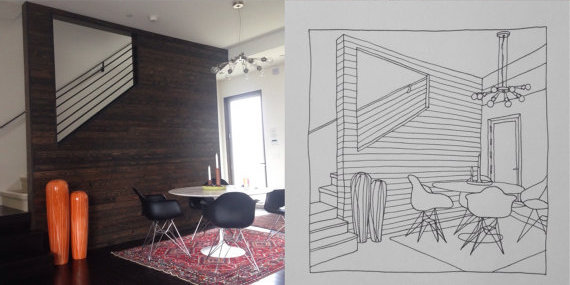
\includegraphics[width=.9\textwidth]{sketch.jpg} 
		\end{column}
		\begin{column}{.5\textwidth}
		Better space complexity, communication complexity, runtime, all at once.
		\end{column}
	\end{columns}	
\end{frame}

\begin{frame}
	\frametitle{binary vector compression}
	We already saw a powerful application of sketching (the MinHash algorithm) to compressing binary vectors. 
	
		\begin{center}
		\vspace{-.5em}
		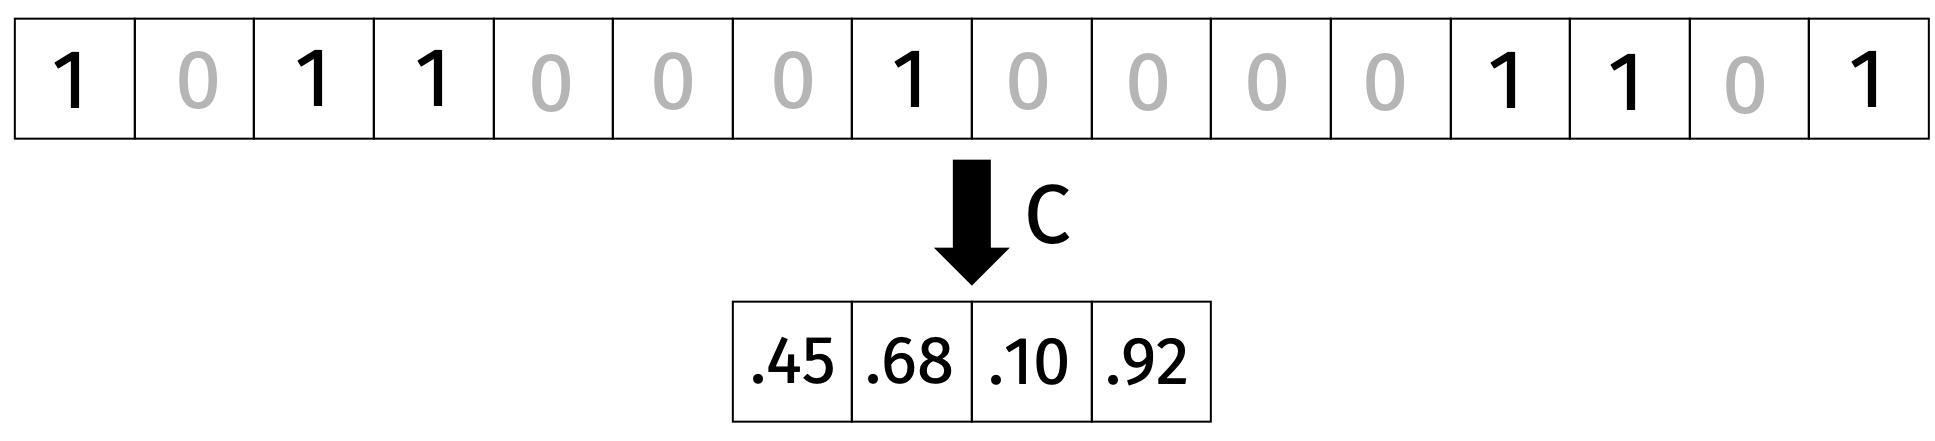
\includegraphics[width=.8\textwidth]{compression.png}
		\vspace{-.5em}
	\end{center}

	Let us estimate the Jaccard similarity between any two binary vectors $\bv{q}$ and $\bv{y}$ using the information in $C(\bv{q})$ and $C(\bv{y})$ alone. 
\end{frame}

\begin{frame}
	\frametitle{today: euclidean dimensionality reduction}
	\begin{center}
		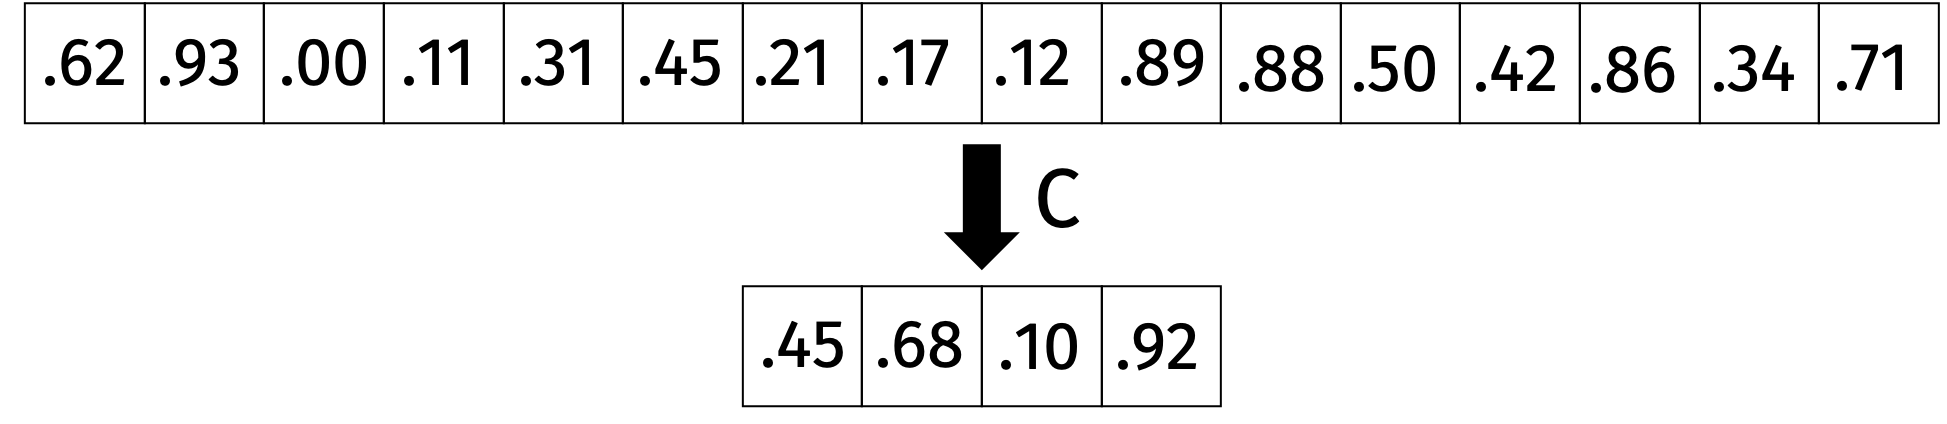
\includegraphics[width=\textwidth]{euclidean_dim_red2.png}
	\end{center}
	Euclidean norm / distance:
	\begin{itemize}
		\item Given $\bv{q} \in \R^d$, $\|\bv{q}\|_2 = \sqrt{\sum_{i=1}^d {q}(i)^2}$.
		\item Given $\bv{q}, \bv{y} \in \R^d$, distance defined as $\|\bv{q} - \bv{y}\|_2$.
	\end{itemize}
	
	\begin{center}
		\alert{
	\textbf{Can we find compact sketches that preserve Euclidean distance, just as we did for Jaccard similarity?}}
	\end{center}
\end{frame}

\begin{frame}
	\frametitle{euclidean dimensionality reduction}
	\begin{lemma}[Johnson-Lindenstrauss, 1984]
		For any set of $n$ data points $\bv{q}_1,\ldots, \bv{q}_n \in \R^d$ there exists a \emph{linear map} $\Pi: \R^d \rightarrow \R^k$ where $k = O\left(\frac{\log n}{\epsilon^2}\right)$ such that \emph{for all $i,j$},
			\begin{align*}
			(1-\epsilon)\|\bv{q}_i - \bv{q}_j\|_2 \leq \|\bs{\Pi}\bv{q}_i - \bs{\Pi}\bv{q}_j\|_2 \leq (1+\epsilon)\|\bv{q}_i - \bv{q}_j\|_2.
			\end{align*}
	\end{lemma}
	\begin{center}
		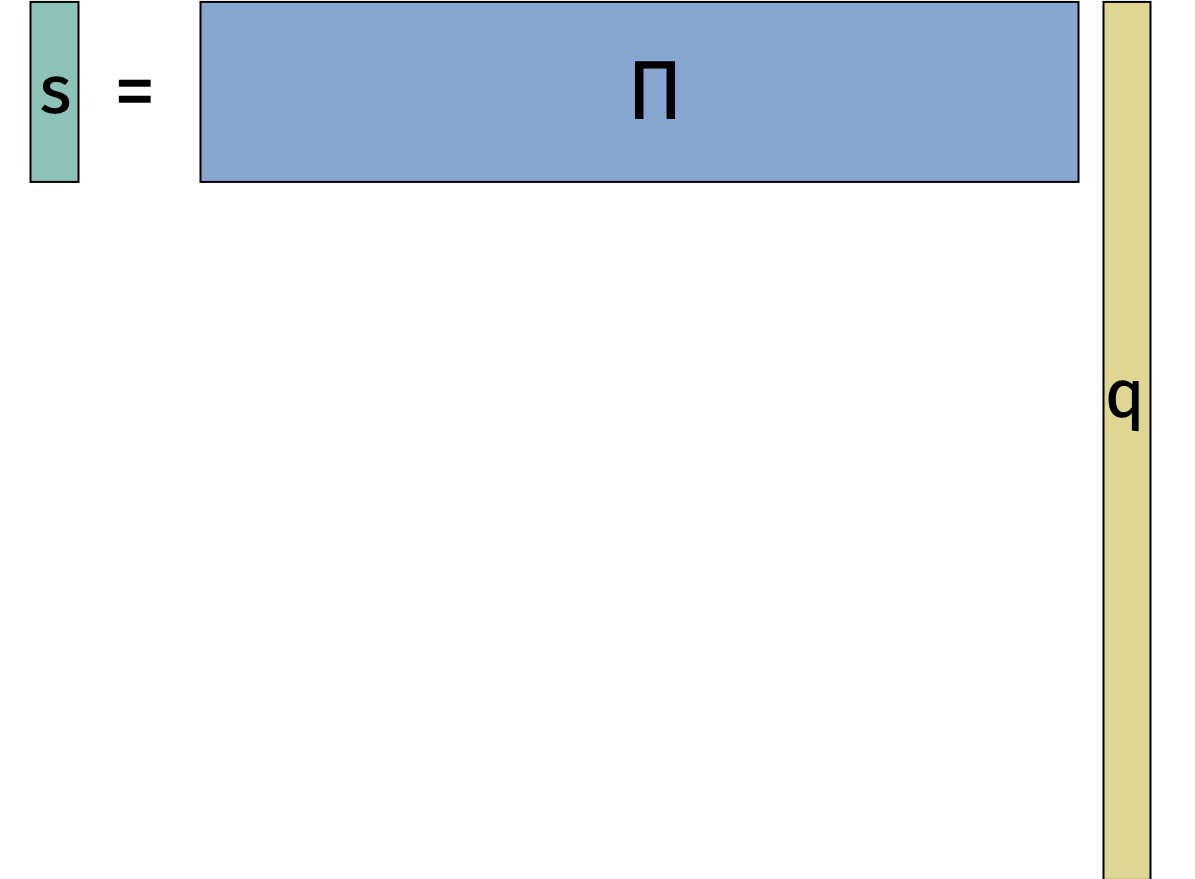
\includegraphics[height=.45\textheight]{jl_sketch.png}
	\end{center}
\end{frame}

\begin{frame}
	\frametitle{euclidean dimensionality reduction}
	\textbf{Please remember:} This is equivalent to: 
	\begin{lemma}[Johnson-Lindenstrauss, 1984]
		For any set of $n$ data points $\bv{q}_1,\ldots, \bv{q}_n \in \R^d$ there exists a \emph{linear map} $\Pi: \R^d \rightarrow \R^k$ where $k = O\left(\frac{\log n}{\epsilon^2}\right)$ such that \emph{for all $i,j$},
		\begin{align*}
			(1-\epsilon)\|\bv{q}_i - \bv{q}_j\|_2^{\mathbf{\alert{2}}} \leq \|\bs{\Pi}\bv{q}_i - \bs{\Pi}\bv{q}_j\|_2^{\mathbf{\alert{2}}} \leq (1+\epsilon)\|\bv{q}_i - \bv{q}_j\|_2^{\mathbf{\alert{2}}}.
		\end{align*}
	\end{lemma}
	because for small $\epsilon$, $(1+\epsilon)^2 = 1 + O(\epsilon)$ and $(1-\epsilon)^2 = 1 - O(\epsilon)$.
\end{frame}

\begin{frame}
	\frametitle{euclidean dimensionality reduction}
	And this is equivalent to:
		\begin{lemma}[Johnson-Lindenstrauss, 1984]
		For any set of $n$ data points $\bv{q}_1,\ldots, \bv{q}_n \in \R^d$ there exists a \emph{linear map} $\Pi: \R^d \rightarrow \R^k$ where $k = O\left(\frac{\log n}{\epsilon^2}\right)$ such that \emph{for all $i,j$},
		\begin{align*}
			(1-\epsilon)\|\bs{\Pi}\bv{q}_i - \bs{\Pi}\bv{q}_j\|_2^{{{2}}} \leq \|\bv{q}_i - \bv{q}_j\|_2^{{{2}}} \leq (1+\epsilon)\|\bs{\Pi}\bv{q}_i - \bs{\Pi}\bv{q}_j\|_2^{{{2}}}.
		\end{align*}
	\end{lemma}
	because for small $\epsilon$, $\frac{1}{1+\epsilon} = 1 - O(\epsilon)$ and $\frac{1}{1-\epsilon} = 1 + O(\epsilon)$.
\end{frame}

\begin{frame}
	\frametitle{euclidean dimensionality reduction}
	\begin{center}
	Remarkably, $\Pi$ can be chosen \emph{completely at random}!
	\end{center}
	\textbf{One possible construction:} Random Gaussian.
	\begin{align*}
		\bs{\Pi}_{i,j} = \frac{1}{\sqrt{k}} \mathcal{N}(0,1)
	\end{align*}
	The map $\bs{\Pi}$ is \textbf{\alert{oblivious to the data set}}. This stands in contrast to e.g. PCA, amoung other differences.
	
	[Indyk, Motwani 1998] [Arriage, Vempala 1999] [Achlioptas 2001] [Dasgupta, Gupta 2003].
	
	Many other possible choices suffice -- you can use random $\{+1,-1\}$ variables, sparse random matrices, pseudorandom $\Pi$. Each with different advantages. 
\end{frame}

\begin{frame}
	\frametitle{randomized jl constructions}
	\begin{center}
		Let $\bs{\Pi} \in \R^{k\times d}$ be chosen so that each entry equals $\frac{1}{\sqrt{k}}  \mathcal{N}(0,1)$.
		
		... or each entry equals $\frac{1}{\sqrt{k}}  \pm 1$ with equal probability.
	\end{center}
	\vspace{1em}
	
	\begin{columns}
		\begin{column}{0.5\textwidth}
			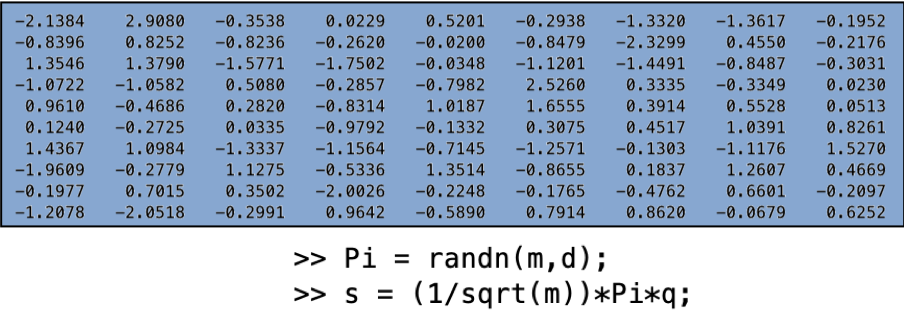
\includegraphics[width=\textwidth]{rand_gauss.png}
		\end{column}
		\begin{column}{0.5\textwidth}
			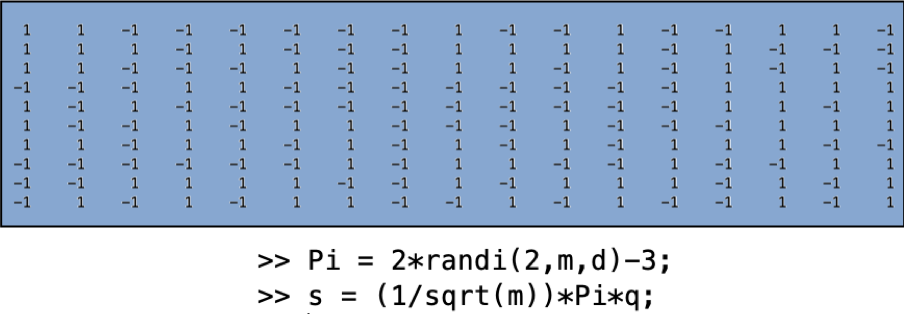
\includegraphics[width=\textwidth]{rand_sign.png}
		\end{column}
	\end{columns}
	
	\begin{center}
		A random orthogonal matrix also works. I.e. with $\Pi\Pi^T = \bv{I}_{k\times k}$. For this reason, the JL operation is often called a ``random projection", even though it technically isn't a projection when entries are i.i.d.
	\end{center}
\end{frame}

\begin{frame}
	\frametitle{random projection}
	\begin{center}
		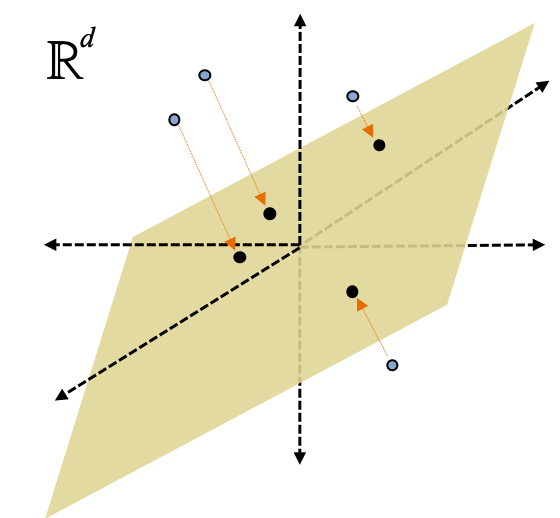
\includegraphics[width=.6\textwidth]{random_projection.png}
	\end{center}
	Intuitively, close points will remain close after projection, and far points will remain far. 
\end{frame}

\begin{frame}
	\frametitle{euclidean dimensionality reduction}
	\textbf{Intermediate result:}
	\begin{lemma}[Distributional JL Lemma]
	Let $\bs{\Pi} \in \R^{k\times d}$ be chosen so that each entry equals $\frac{1}{\sqrt{k}}  \mathcal{N}(0,1)$, where $\mathcal{N}(0,1)$ denotes a standard Gaussian random variable. 
	
	If we choose $k = O\left(\frac{\log(1/\delta)}{\epsilon^2}\right)$, then for \emph{any vector $\bv{x}$}, with probability $(1-\delta)$:
	\begin{align*}
		(1-\epsilon)\|\bv{x}\|_2^2 \leq \|\bs{\Pi}\bv{x}\|_2^2 \leq (1+\epsilon) \|\bv{x}\|_2^2
	\end{align*}
	\end{lemma}

\begin{center}\alert{
	Given this lemma, how do we prove the traditional Johnson-Lindenstrauss lemma?}
\end{center}
\end{frame}

\begin{frame}
	\frametitle{jl from distributional jl}
	We have a set of vectors $\bv{q}_1, \ldots, \bv{q}_n$. Fix $i,j \in 1,\ldots, n$. 
	
	Let $\bv{x} = \bv{q}_i - \bv{q}_j$. By linearity, $\bs{\Pi}\bv{x} = \bs{\Pi}(\bv{q}_i - \bv{q}_j) = \bs{\Pi}\bv{q}_i - \bs{\Pi}\bv{q}_j$.
	
	By the Distributional JL Lemma, with probability $1-\delta$,
	\begin{align*}
		(1-\epsilon)\|\bv{q}_i - \bv{q}_j\|_2 \leq \|\bs{\Pi}\bv{q}_i - \bs{\Pi}\bv{q}_j\|_2 \leq (1+\epsilon) \|\bv{q}_i - \bv{q}_j\|_2.
	\end{align*}
	Finally, set $\delta = \frac{1}{n^2}$. Since there are $< n^2$ total $i,j$ pairs, by a union bound we have that with probability $9/10$, the above will hold \emph{for all} $i,j$, as long as we compress to:

	\begin{align*}
		k = O\left(\frac{\log(1/(1/n^2))}{\epsilon^2}\right) = O\left(\frac{\log n}{\epsilon^2}\right) \text{ dimensions.}\qed
	\end{align*}
	
\end{frame}

\begin{frame}
	\frametitle{proof of distributional jl}
	Want to argue that, with probability $(1-\delta)$,
	\begin{align*}
	(1-\epsilon)\|\bv{x}\|_2^2 \leq |\bs{\Pi}\bv{x}\|_2^2 \leq (1+\epsilon)\|\bv{x}\|_2^2 
	\end{align*}
	
	\begin{center}
	\alert{\textbf{Claim}: $\E \|\bs{\Pi} \bv{x} \|_2^2 = \|\bv{x}\|_2^2.$}
	\end{center}

\vspace{-1em}
Some notation:
\begin{center}
	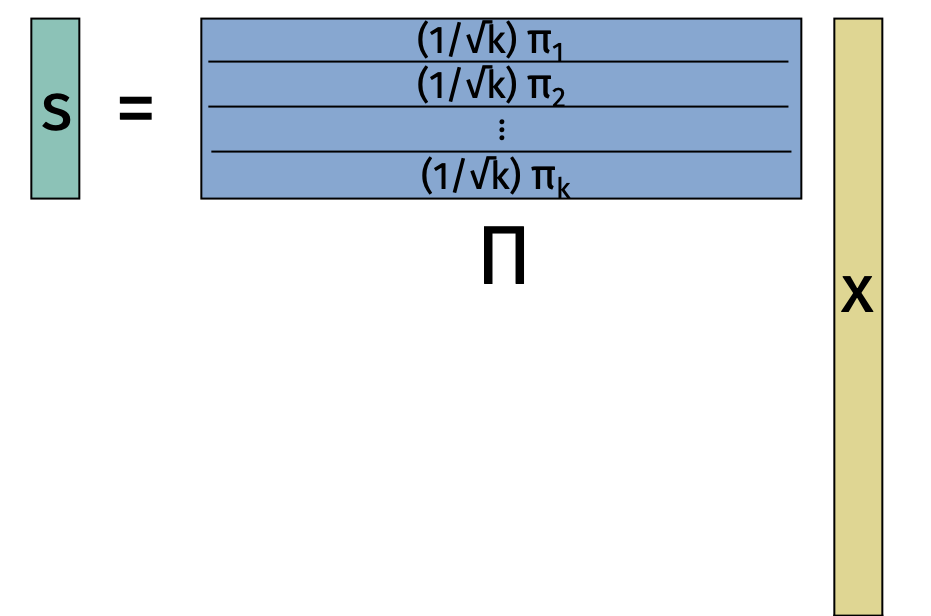
\includegraphics[width=.6\textwidth]{jl_notation.png}
	
	So each $\bs{\pi}_i$ contains $\mathcal{N}(0,1)$ entries. 
\end{center}
\end{frame}

\begin{frame}
	\frametitle{proof of distributional jl}
	\begin{align*}
		\|\bs{\Pi} \bv{x} \|_2^2 = \sum_i^k \bv{s}(i)^2 = \sum_i^k \left(\frac{1}{\sqrt{k}}\langle\bs{\pi}_i,\bv{x}\rangle\right)^2 = \frac{1}{k}\sum_i^k \left(\langle\bs{\pi}_i,\bv{x}\rangle\right)^2 
	\end{align*}
	\begin{align*}
		\E\left[\|\bs{\Pi} \bv{x} \|_2^2 \right] &= \frac{1}{k}\sum_i^k \E\left[\left(\langle\bs{\pi}_i,\bv{x}\rangle\right)^2 \right] \\
		& =\E\left[\left(\langle\bs{\pi}_i,\bv{x}\rangle\right)^2 \right] 
	\end{align*}
	\vspace{4em}
	\begin{block}{\vspace*{-3ex}}
		\small \textbf{Goal}: Prove $\E \|\bs{\Pi} \bv{x} \|_2^2 = \|\bv{x}\|_2^2$.
	\end{block}
\end{frame}

\begin{frame}
	\frametitle{proof of distributional jl}	
	\begin{align*}
		\langle\bs{\pi}_i,\bv{x}\rangle = Z_1\cdot\bv{x}(1) + Z_2\cdot\bv{x}(2)  +  \ldots + Z_d\cdot\bv{x}(d)
	\end{align*}
	where each $Z_1, \ldots, Z_d$ is a standard normal $\mathcal{N}(0,1)$ random variable. 
	
	This implies that $Z_i \cdot\bv{x}(i)$ is a normal $\mathcal{N}(0,\bv{x}(i)^2)$ random variable.
	
	\vspace{5em}
	\begin{block}{\vspace*{-3ex}}
		\small \textbf{Goal}: Prove $\E \|\bs{\Pi} \bv{x} \|_2^2 = \|\bv{x}\|_2^2$. Established: $\E \|\bs{\Pi} \bv{x} \|_2^2 = \E\left[\left(\langle\bs{\pi}_i,\bv{x}\rangle\right)^2 \right]$
	\end{block}
\end{frame}

\begin{frame}[t]
	\frametitle{stable random variables}
	\textbf{What type of random variable is $\langle\bs{\pi}_i,\bv{x}\rangle$?}
		\begin{fact}[Stability of Gaussian random variables]
			\begin{align*}
			\mathcal{N}(\mu_1, \sigma_1^2) + \mathcal{N}(\mu_2, \sigma_2^2) =  \mathcal{N}(\mu_1 + \mu_2, \sigma_1^2 + \sigma_2^2)
			\end{align*}
		\end{fact}
		\begin{align*}
			\langle\bs{\pi}_i,\bv{x}\rangle &= \mathcal{N}(0,\bv{x}(1)^2) + \mathcal{N}(0,\bv{x}(2)^2) + \ldots + \mathcal{N}(0,\bv{x}(d)^2) \\ &= \mathcal{N}(0,\|\bv{x}\|_2^2). 
		\end{align*}
	
	So $\E \|\bs{\Pi} \bv{x} \|_2^2 = \E\left[\left(\langle\bs{\pi}_i,\bv{x}\rangle\right)^2 \right] = \|\bv{x}\|_2^2$, as desired.
\end{frame}

\begin{frame}
	\frametitle{proof of distributional jl}
	Want to argue that, with probability $(1-\delta)$,
	\begin{align*}
		(1-\epsilon)\|\bv{x}\|_2^2 \leq \|\bs{\Pi}\bv{x}\|_2^2 \leq (1+\epsilon)\|\bv{x}\|_2^2 
	\end{align*}
	
	\begin{enumerate}
		\item $\E \|\bs{\Pi} \bv{x} \|_2^2 = \|\bv{x}\|_2^2$.
		\item Need to use a concentration bound.
	\end{enumerate}
	\begin{align*}
		\|\bs{\Pi} \bv{x} \|_2^2 = \frac{1}{k}\sum_{i=1}^k \left(\langle\bs{\pi}_i,\bv{x}\rangle\right)^2 = \frac{1}{k}\sum_{i=1}^k \mathcal{N}(0,\|\bv{x}\|_2^2)
	\end{align*}
\alert{``Chi-squared random variable with $k$ degrees of freedom.''}
\end{frame}

\begin{frame}[t]
	\frametitle{concentration of chi-squared random variables}
	\begin{lemma} Let $Z$ be a Chi-squared random variable with $k$ degrees of freedom. 
		\begin{align*}
		\Pr[|\E Z - Z| \geq \epsilon \E Z] \leq 2 e^{-k\epsilon^2/8}
		\end{align*}
	\end{lemma}

\vspace{8em}
	\begin{block}{\vspace*{-3ex}}
	\small \textbf{Goal}: Prove $\|\bs{\Pi} \bv{x} \|_2^2$ concentrates within $1 \pm \epsilon$ of its expectation, which equals $\|\bv{x} \|_2^2$.
\end{block}
\end{frame}

\begin{frame}[t]
	\frametitle{sample application}
	\textbf{k-means clustering}: Give data points $\bv{a}_1,\ldots, \bv{a}_n \in \R^d$, find centers $\bs{\mu}_1, \ldots, \bs{\mu}_k\in \R^d$ to minimize:
	\begin{align*}
		Cost(\bs{\mu}_1,\ldots, \bs{\mu}_k) = \sum_{i=1}^n \min_{j = 1,\ldots,k} \|\bs{\mu}_j - \bv{X}_i\|_2^2
	\end{align*}
	\begin{center}
		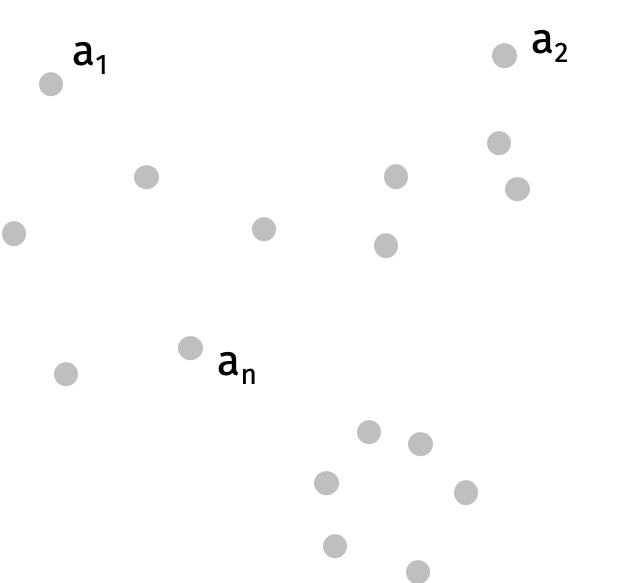
\includegraphics[width=.5\textwidth]{kmeans1.png}
	\end{center}
\end{frame}
\begin{frame}[t]
	\frametitle{sample application}
	\textbf{k-means clustering}: Give data points $\bv{a}_1,\ldots, \bv{a}_n \in \R^d$, find centers $\bs{\mu}_1, \ldots, \bs{\mu}_k\in \R^d$ to minimize:
	\begin{align*}
		Cost(\bs{\mu}_1,\ldots, \bs{\mu}_k) = \sum_{i=1}^n \min_{j = 1,\ldots,k} \|\bs{\mu}_j - \bv{X}_i\|_2^2
	\end{align*}
	\begin{center}
		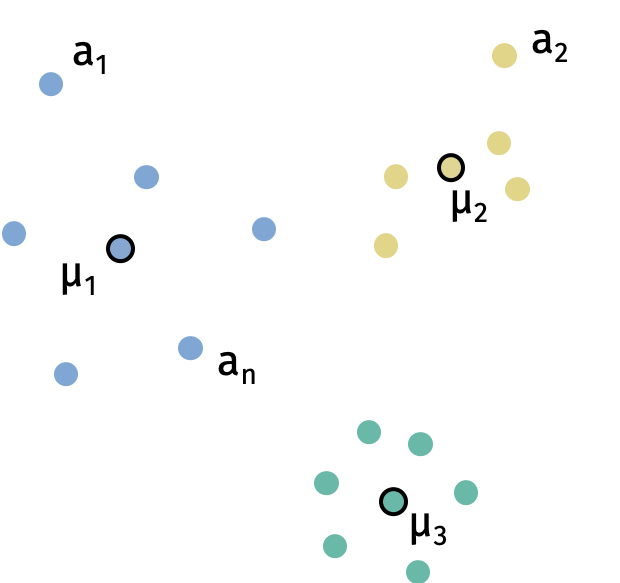
\includegraphics[width=.5\textwidth]{kmeans2.png}
	\end{center}
\end{frame}
\begin{frame}[t]
	\frametitle{sample application}
	\textbf{k-means clustering}: Give data points $\bv{a}_1,\ldots, \bv{a}_n \in \R^d$, find centers $\bs{\mu}_1, \ldots, \bs{\mu}_k\in \R^d$ to minimize:
	\begin{align*}
		Cost(\bs{\mu}_1,\ldots, \bs{\mu}_k) = \sum_{i=1}^n \min_{j = 1,\ldots,k} \|\bs{\mu}_j - \bv{a}_i\|_2^2
	\end{align*}
	\begin{center}
		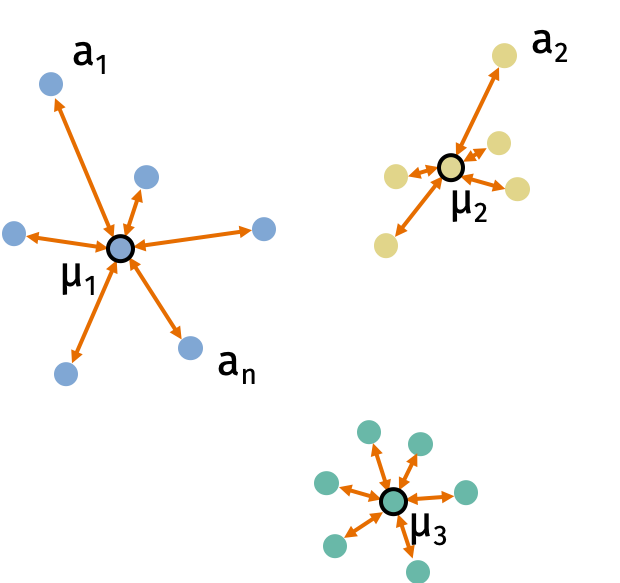
\includegraphics[width=.5\textwidth]{kmeans3.png}
	\end{center}
\end{frame}

\begin{frame}[t]
	\frametitle{k-means clustering}
	NP hard to solve exactly, but there are many good approximation algorithms. All depend at least linearly on the dimension $d$. 
	
	\textbf{Approximation scheme}: Find clusters $\tilde{C}_1, \ldots, \tilde{C}_k$ for the $k = O\left(\frac{\log n}{\epsilon^2}\right)$ dimension data set $\bs{\Pi}\bv{a}_1, \ldots, \bs{\Pi}\bv{a}_n.$
	
	\vspace{-3em}
	\begin{center}
		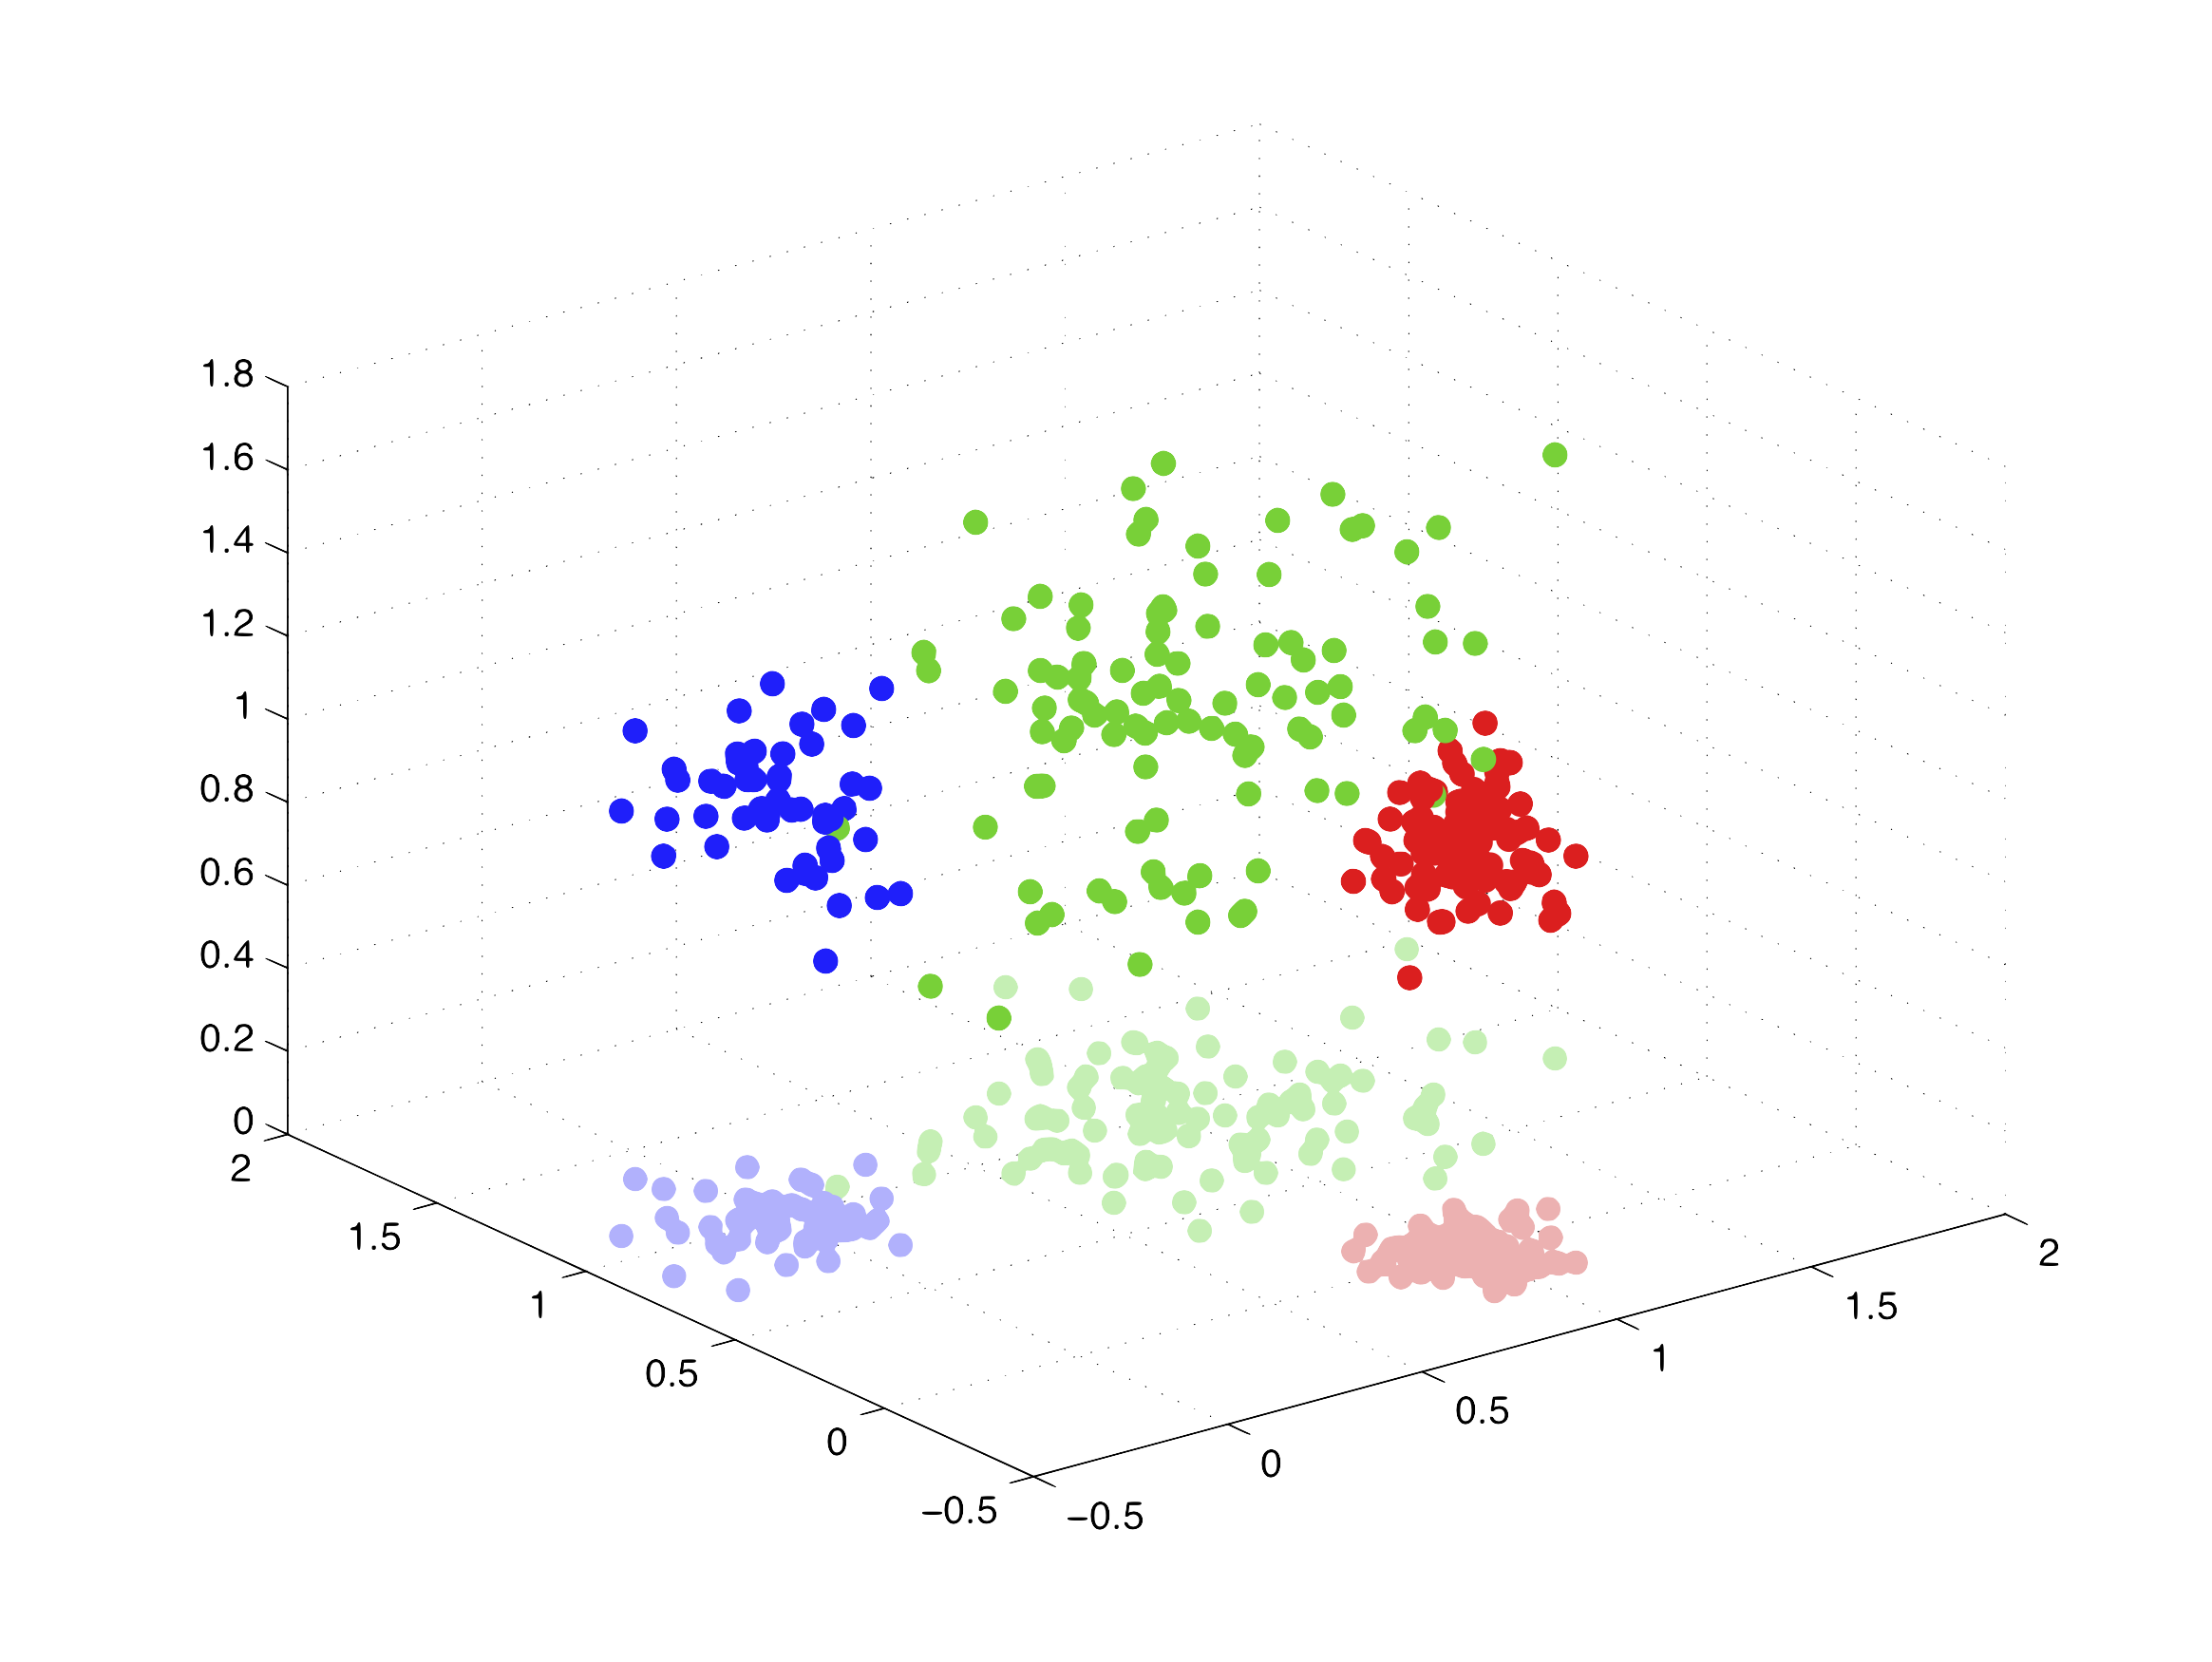
\includegraphics[width=.6\textwidth]{clustering_projected.png}
	\end{center}
	\vspace{-2em}
Argue these clusters are near optimal for $\bv{a}_1, \ldots, \bv{a}_n$.
\end{frame}

\begin{frame}[t]
	\frametitle{k-means clustering}
	\textbf{Equivalent formulation}: Find clusters $C_1, \ldots, C_k \subseteq \{1, \ldots, n\}$ to minimize:
	\begin{align*}
	Cost(C_1,\ldots, C_k) = \sum_{j=1}^k \frac{1}{2|C_j|}\sum_{u,v\in C_j} \|\bv{a}_u - \bv{a}_v\|_2^2.
	\end{align*}
\vspace{-1em}
	\begin{center}
	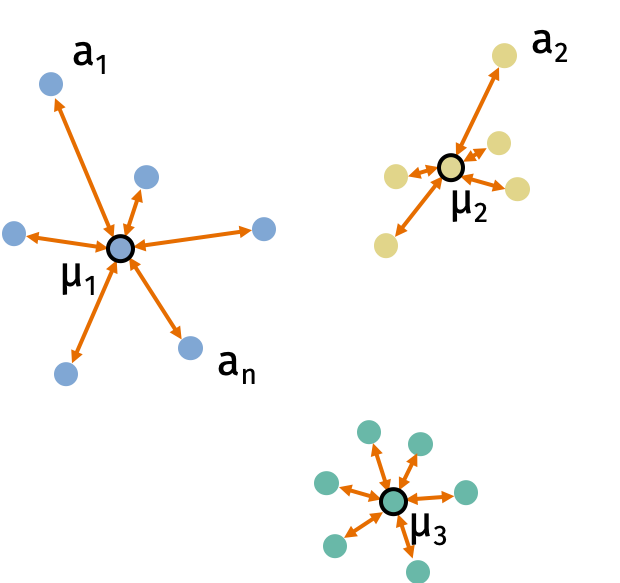
\includegraphics[width=.5\textwidth]{kmeans3.png}
	\end{center}
\end{frame}
\begin{frame}[t]
	\frametitle{k-means clustering}
	\textbf{Equivalent formulation}: Find clusters $C_1, \ldots, C_k \subseteq \{1, \ldots, n\}$ to minimize:
	\begin{align*}
		Cost(C_1,\ldots, C_k) = \sum_{j=1}^k \frac{1}{2|C_j|}\sum_{u,v\in C_j} \|\bv{a}_u - \bv{a}_v\|_2^2.
	\end{align*}
\vspace{-1em}
	\begin{center}
		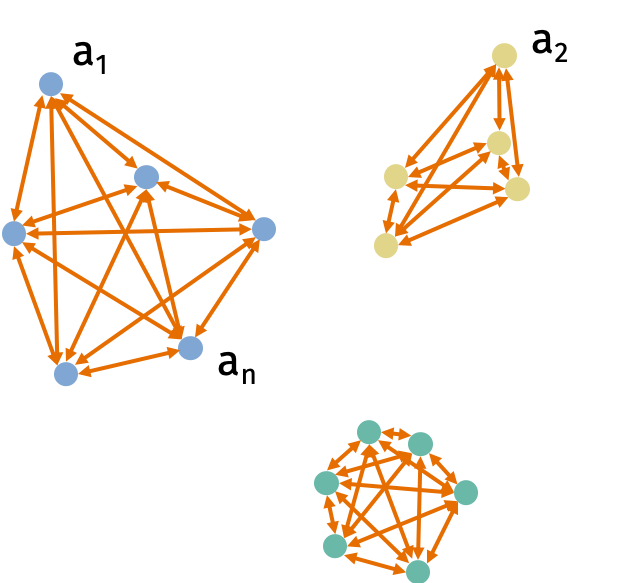
\includegraphics[width=.5\textwidth]{kmeans4.png}
	\end{center}
\textbf{Exercise:} Prove this to your self.
\end{frame}



\begin{frame}[t]
	\frametitle{k-means clustering}
	\begin{align*}
	Cost(C_1,\ldots, C_k) &= \sum_{j=1}^k \frac{1}{2|C_j|}\sum_{u,v\in C_j} \|\bv{a}_u - \bv{a}_v\|_2^2 \\
	\widetilde{Cost}(C_1,\ldots, C_k) &= \sum_{j=1}^k \frac{1}{2|C_j|}\sum_{u,v\in C_j} \|\Pi\bv{a}_u - \Pi\bv{a}_v\|_2^2
	\end{align*}

\end{frame}

\begin{frame}[t]
	\frametitle{k-means clustering}
	Let $Cost^* = \min Cost(C_1,\ldots, C_k)$ and $\widetilde{Cost}^* = \min \widetilde{Cost}(C_1,\ldots, C_k)$.
	
	\textbf{Claim:} $(1-\epsilon) {Cost}^* \leq \widetilde{Cost}^* \leq (1+\epsilon) {Cost}^*$.
\end{frame}

\begin{frame}[t]
	\frametitle{k-means clustering}
	Suppose we use an approximation algorithm to find clusters $B_1, \ldots, B_k$ such that:
	\begin{align*}
		\widetilde{Cost}(B_1,\ldots, B_k) \leq (1+\alpha)\widetilde{Cost}^*
	\end{align*}

	Then: 
	\begin{align*}
	{Cost}(B_1,\ldots, B_k) &\leq \frac{1}{1-\epsilon}\widetilde{Cost}(B_1,\ldots, B_k) \\
	&\leq (1+\alpha)(1+O(\epsilon))\widetilde{Cost}^*\\
	&\leq (1+\alpha)(1+O(\epsilon))(1+\epsilon){Cost}^*\\
	&= \alert{1 + O(\alpha + \epsilon){Cost}^*}
	\end{align*}
\end{frame}

\begin{frame}
	\frametitle{connection to last lecture}
	If high dimensional geometry is so different from low-dimensional geometry, why is \emph{dimensionality reduction possible?} Doesn't Johnson-Lindenstrauss tell us that high-dimensional geometry can be approximated in low dimensions?
\end{frame}

\begin{frame}
	\frametitle{connection to dimensionality reduction}
	\textbf{Hard case:} $\bv{x}_1, \ldots, \bv{x}_n \in \R^d$ are all mutually orthogonal unit vectors: 
	\begin{align*}
	\|\bv{x}_i - \bv{x}_j\|_2^2 &= 2 & &\text{for all $i,j$.}  
	\end{align*}
	
	From our result earlier, in $O(\log n /\epsilon^2)$ dimensions, there exists $2^{O(\epsilon^2\cdot \log n /\epsilon^2)} \geq n $ unit vectors that are close to mutually orthogonal.
	
	 $O(\log n /\epsilon^2)$ = \emph{just enough} dimensions. 
\end{frame}

\end{document} 








